The purpose of this case is to test the calculation of exceedance curves for the downtime, or business-interruption losses for an asset. The loss due to downtime, or business-interruption for the asset used in this case is $2,000 / month$. Downtime losses are usually specified per unit time the asset will be unavailable for occupancy or use. Table~\ref{tab:vf-ln-tax1-dnt} shows the mean loss ratios and corresponding coefficients of variation for the downtime vulnerability function used in this test case. Apart from the change in the vulnerability function and value, the calculation procedure remains the same as described in Case~1d.

The loss curve calculated using the implementation of the calculator in Julia is compared with that produced by OpenQuake in Figure~\ref{fig:lc-ebr-2c}.

\begin{figure}[htbp]
\centering
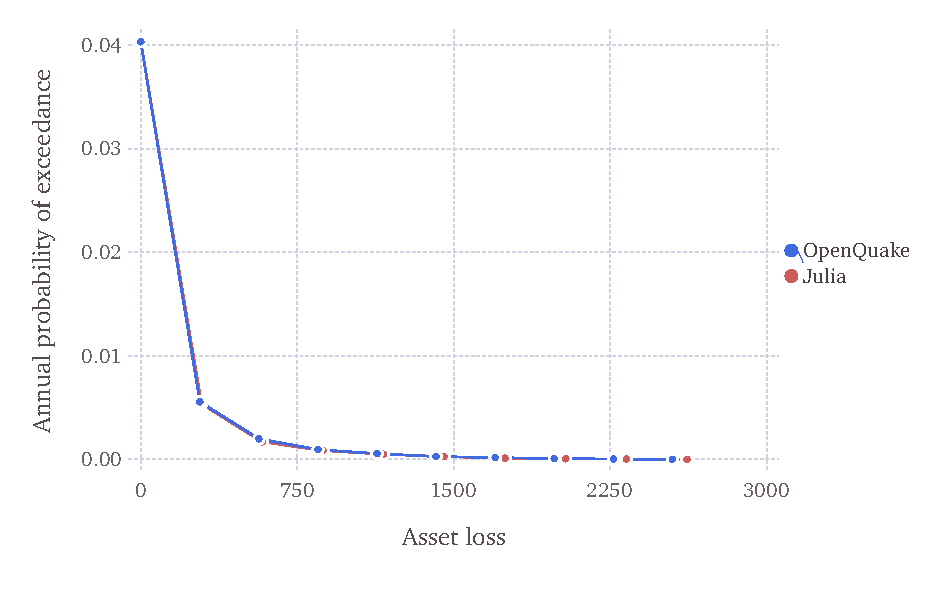
\includegraphics[width=12cm]{qareport/figures/fig-lc-ebr-2c}
\caption{Loss curve comparison for event based risk test case 2c}
\label{fig:lc-ebr-2c}
\end{figure}